%! TEX root = ../master.tex

\subsection{Hausdorff spaces}

\begin{problem}
	Let $Y$ be a topological space with the trivial topology.
	Show that every sequence in $Y$ converges to every point in $Y$.
\end{problem}

\begin{solution}
	Let $ \{ y_i \}_{i=1}^\infty$ be some sequence in $Y$ and $y \in Y$.
	Then $U = Y$ is a neighbourhood of $y$ (infact the only one)
	such that $y_i \subset U$ for all $i \geq 1$ and hence
	$y_i \to y$.
\end{solution}

\begin{remark}
	This problem shows that, although flexible,
	topological spaces can contradict a lot of intuition that we have
	built looking at metric spaces.
\end{remark}

\begin{definition}[Hausdorff spaces]
	Let $X$ be a topological space.
	We say that $X$ is a \textbf{Hausdorff space}
	if for all distinct points $p$ and $q$ in $X$,
	there exists the respective neighbourhoods
	$U$ and $V$ such that
	$U \cap V = \emptyset$.
\end{definition}

\begin{example}[]
	\hfill
	\begin{enumerate}
		\item All metric spaces are Hausdorff.
		\item All disrete spaces are Hausdorff.
		\item Every open subset of a Hausdorff space is Hausdorff.
	\end{enumerate}
\end{example}

\begin{problem}
	Suppose $X$ is a topological space
	and for every point $p$ in $X$ there exists a continuous function
	$f_x: X \to \R$ such that $ \left( f_x \right)^{-1}(0) = \left\{ p \right\}$.
	Show that $X$ is Hausdorff.
\end{problem}

\begin{proof}
	%todo
\end{proof}

\begin{example}[]
	The trivial topology on any set with more than one element is non-Hausdorff.
	As all metric spaces are Hausdorff, it follows that non-Hausdorff spaces are
	not metrizable.
\end{example}

\begin{proposition}[]
	Let $X$ be a Hausdorff space.
	\begin{enumerate}
		\item Every finite subset of $X$ is closed.
		\item If a sequence $ \left\{ p_i \right\} $ in $X$
			converges to a limit $p \in X$, the limit is unique.
	\end{enumerate}
\end{proposition}

\begin{proof}
	\hfill
	\begin{enumerate}
		\item The idea of this proof is to show that for a closed finite subset
			$A \subset X$, the singleton sets must be open and thus must be
			closed. The finite union of closed subsets is closed.

		\item This proof is a simple contradiction following from the basic
			property of a Hausdorff space.
	\end{enumerate}
\end{proof}

\begin{problem}
	Show that the only topology that is Hausdorff on a finite set is the discrete
	topology.
\end{problem}

\begin{proof}
	Suppose $X$ is a finite Hausdorff space.
	Let $x \in X$ be a fixed point.
	Now for every other point in $X$ there exists disjoint
	neighbourhoods of both points.
	Taking the union of all of the neighbourhoods of $x$
	gives us $\{x\}$, which is open.
	So on a finite Hausdroff space, the singleton sets must be open.
	This generates the discrete toplogy.
\end{proof}

\begin{proposition}[]
	Suppose $X$ is a Hausdorff space and $A \subset X$.
	If $p \in A$ is a limit point of $A$, 
	then every neighbourhood of $p$ contains infinitely many points of $A$.
\end{proposition}

\begin{proof}
	See Figure \ref{fig:topology-diagram-1} to convice yourself.
	Let $M$ be some neighbourhood of $p$ and suppose $a_1, a_2, \ldots, a_n$
	be the points of $M$ in $A$
	(we are assuming there are finitely many for a contradiction).
	Now as $X$ is Hausdorff, we can separate $p$ and $a_i$ with neighbourhoods.
	Taking the union of all the neighbourhoods of $p$ we get $U$, which is open.
	But by assumption all neighbourhoods of $p$ must contain a point in $A$;
	a contradiction.
\end{proof}

\begin{figure}[htpb]
	\centering
	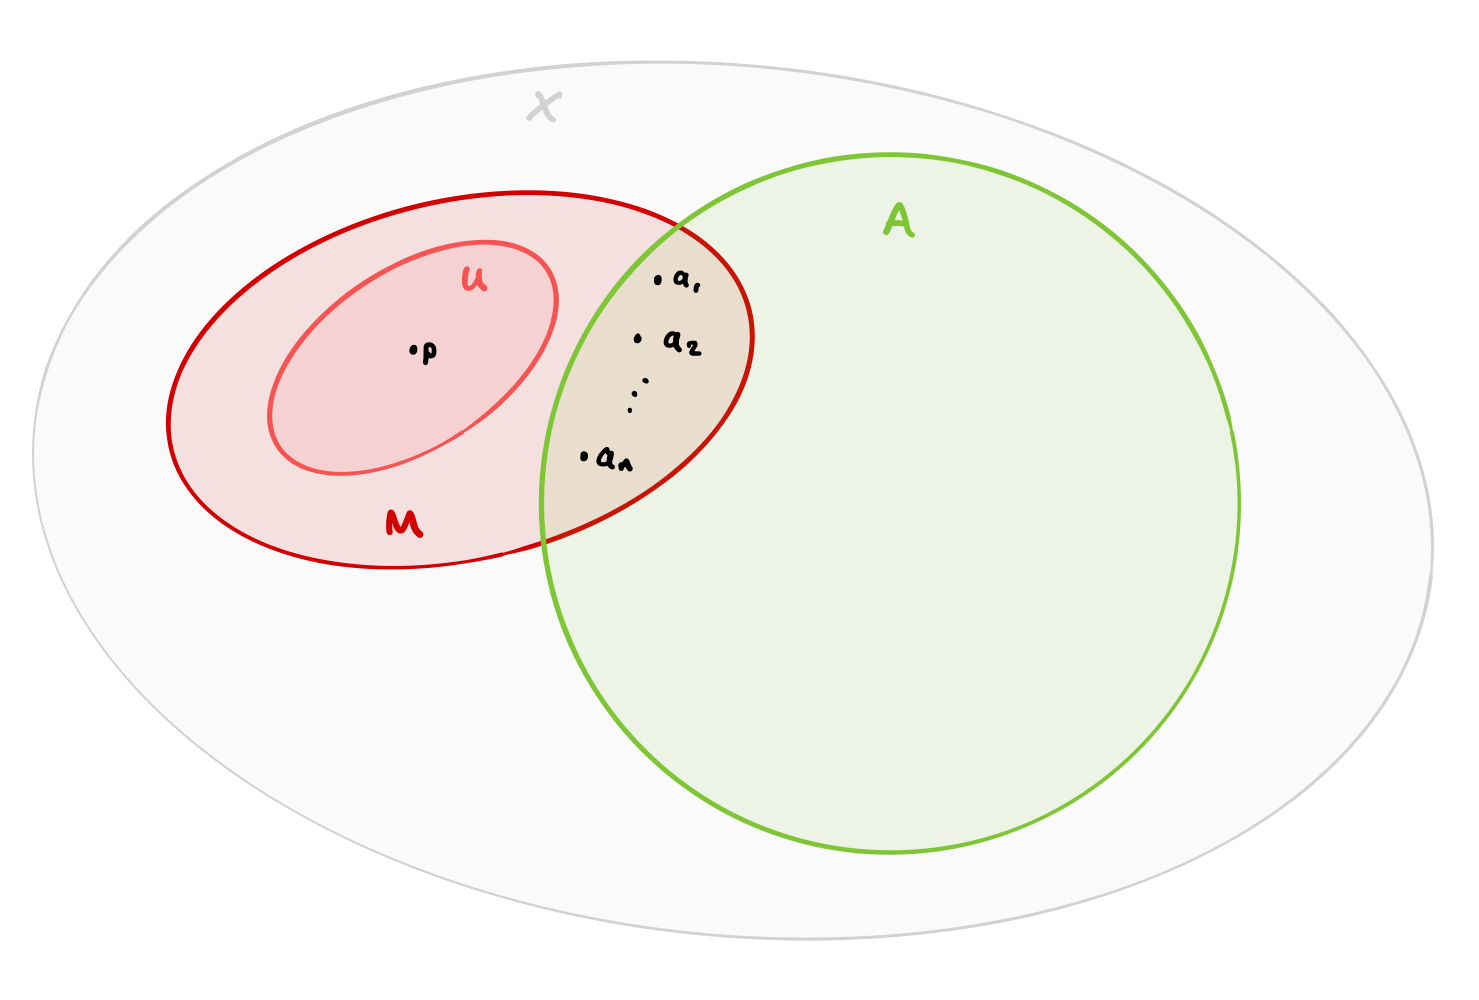
\includegraphics[width=0.8\linewidth]{topology/images/diagram-1.png}
	\caption{}
	\label{fig:topology-diagram-1}
\end{figure}
